\chapter*{Results}
\label{ch:results}
% The performances of the models were evaluated using the
% \texttt{classification\_report} function from the \texttt{scikit-learn} library. 
% This function is particularly useful as it offers an overview of key evaluation
% metrics commonly used in Machine Learning, i.e. accuracy, precision, recall,
% and F1-score.\\
The performance metrics taken into account for evaluation are the following:
accuracy, precision, recall, and F1-score. Taking all of them into account
is crucial to accurately evaluate how well each model performs.

For the static models implemented in this project, the classification report
revealed an accuracy of 34\% for the Random Forest algorithm and 43\% for SVM. 
These results can be considered reasonable, given that the task at hand is a
multi-class classification problem with 8 classes.\\

Neural Networks' performances were not \textbf{AGGIUNGERE ALTRO}\\

In order to gain insights into the features influencing the models' classification decisions, an explainability analysis was conducted.
The aim of this step is indeed to interpret, in understandable terms, certain predictions made by the SVC classifier for the target variable label using a smaller subset of the dataset. 
The analysis employed LIME, a post hoc model-agnostic technique designed to explain a learning model. Instance-based explanations were generated in order to illustrate the reasons for the classification of song's stanzas.
LIME treats the model as black box and constructs a simpler surrogate model to approximate the local behavior of the original model for the prediction of the instance's label. 
The surrogate model is trained on an approximated version of the original dataset, where the instance's values are perturbed. Feature importance scores are then calculated, 
indicating how much a feature was relevant in the prediction of a class label of a data point; these scores show whether a feature increased the probability of that class or if it increased the probability prediction of other classes.

An interesting aspect of the explainability analysis is the visualization of the results.
The \textbf{left section} of the graph in Figure~\ref{fig:expl} displays the predicted probabilities for each class. In the \textbf{center section}
feature importances are ranked from most to least relevant and divided into two groups: on the right
features with a positive influence on the predicted label; on the left, those with a negative influence that suggest the model should consider other classes.
The \textbf{right section} of the graph highlights the values of the most important
features, wusing bright colors to indicate features with a positive influence on the prediction.

\begin{figure}[H]
    \centering
    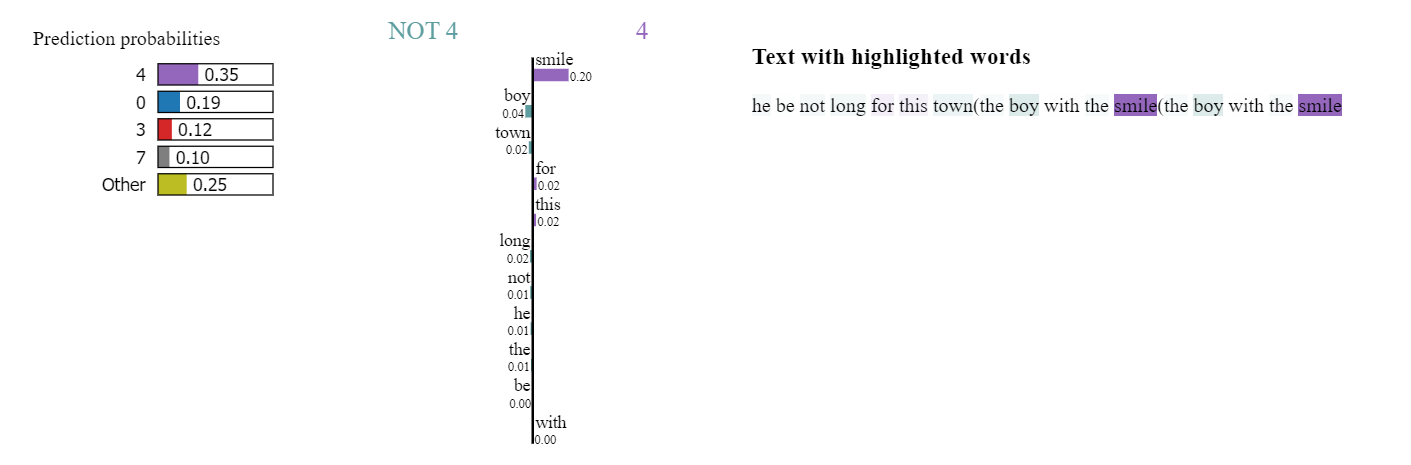
\includegraphics[scale= 0.55]{pictures/expl.png}
    \caption{Explainability - visualization}
    \label{fig:expl}
\end{figure}

The figure above illustrates a prediction where the model assigned the label \texttt{joy} to the stanza under analysis, but the correct label, assigned by the ALBERT model (as mentioned in the \textit{Methods} section), was \texttt{sadness}.
However, the word "smile" which is brighty highlighted, intuitively suggests that "joy" might be a more plausible class for this stanza, even one that ALBERT could reasonably assign. 
This observation raises a critical issue: the transfer learning approach used to create the ground truth appears to have some limitations; in some instances the SVC model assigns a label that seems more contextually appropriate for the stanza, 
yet it differs from the supposedly correct label provided by ALBERT.
